\listfiles
%%%%%%%%%%%%%%%%%%%%%%%%%%%%%%%%%%%%%%%%%
% Masters/Doctoral Thesis 
% LaTeX Template
% Version 2.4 (22/11/16)
%
% This template has been downloaded from:
% http://www.LaTeXTemplates.com
%
% Version 2.x major modifications by:
% Vel (vel@latextemplates.com)
%
% This template is based on a template by:
% Steve Gunn (http://users.ecs.soton.ac.uk/srg/softwaretools/document/templates/)
% Sunil Patel (http://www.sunilpatel.co.uk/thesis-template/)
%
% Template license:
% CC BY-NC-SA 3.0 (http://creativecommons.org/licenses/by-nc-sa/3.0/)
%
%%%%%%%%%%%%%%%%%%%%%%%%%%%%%%%%%%%%%%%%%

%----------------------------------------------------------------------------------------
%	PACKAGES AND OTHER DOCUMENT CONFIGURATIONS
%----------------------------------------------------------------------------------------

\documentclass[
11pt, % The default document font size, options: 10pt, 11pt, 12pt
oneside, % Two side (alternating margins) for binding by default, uncomment to switch to one side
english, % ngerman for German
singlespacing, % Single line spacing, alternatives: onehalfspacing or doublespacing
% for thesis review - use doublespacing, for final version use singlespacing
%draft, % Uncomment to enable draft mode (no pictures, no links, overfull hboxes indicated)
%nolistspacing, % If the document is onehalfspacing or doublespacing, uncomment this to set spacing in lists to single
%liststotoc, % Uncomment to add the list of figures/tables/etc to the table of contents
%toctotoc, % Uncomment to add the main table of contents to the table of contents
%parskip, % Uncomment to add space between paragraphs
%nohyperref, % Uncomment to not load the hyperref package
headsepline, % Uncomment to get a line under the header
%chapterinoneline, % Uncomment to place the chapter title next to the number on one line
%consistentlayout, % Uncomment to change the layout of the declaration, abstract and acknowledgements pages to match the default layout
]{MastersDoctoralThesis} % The class file specifying the document structure

\usepackage[utf8]{inputenc} % Required for inputting international characters
\usepackage[T1]{fontenc} % Output font encoding for international characters

\usepackage{palatino} % Use the Palatino font by default
\usepackage[backend=bibtex,style=numeric,citestyle=numeric,natbib=true]{biblatex} % Use the bibtex backend with the authoryear citation style (which resembles APA)

\addbibresource{example.bib} % The filename of the bibliography

\usepackage[autostyle=true]{csquotes} % Required to generate language-dependent quotes in the bibliography

%----------------------------------------------------------------------------------------
%	MARGIN SETTINGS
%----------------------------------------------------------------------------------------
\newtheorem{theorem}{Theorem}[section]
\geometry{
	paper=a4paper, % Change to letterpaper for US letter
	inner=2.5cm, % Inner margin
	outer=3.8cm, % Outer margin
	bindingoffset=.5cm, % Binding offset
	top=1.5cm, % Top margin
	bottom=1.5cm, % Bottom margin
	%showframe, % Uncomment to show how the type block is set on the page
}

%----------------------------------------------------------------------------------------
%	THESIS INFORMATION
%----------------------------------------------------------------------------------------

\thesistitle{Deception Detection By Autonomous Agent Based On Speech} % Your thesis title, this is used in the title and abstract, print it elsewhere with \ttitle
\supervisor{Dr. Amos  \textsc{Azaria}} % Your supervisor's name, this is used in the title page, print it elsewhere with \supname
\examiner{} % Your examiner's name, this is not currently used anywhere in the template, print it elsewhere with \examname
\degree{Master} % Your degree name, this is used in the title page and abstract, print it elsewhere with \degreename
\author{Evgeny \textsc{Hershkovitch Neiterman}} % Your name, this is used in the title page and abstract, print it elsewhere with \authorname
\addresses{} % Your address, this is not currently used anywhere in the template, print it elsewhere with \addressname

\subject{Computer Science} % Your subject area, this is not currently used anywhere in the template, print it elsewhere with \subjectname
\keywords{Keyword1, Keyword2, Keyword3} % Keywords for your thesis, this is not currently used anywhere in the template, print it elsewhere with \keywordnames
\university{\href{http://www.university.com}{Ariel University}} % Your university's name and URL, this is used in the title page and abstract, print it elsewhere with \univname
\department{\href{http://department.university.com}{Department of Computer Science}} % Your department's name and URL, this is used in the title page and abstract, print it elsewhere with \deptname
\group{\href{http://researchgroup.university.com}{ }} % Your research group's name and URL, this is used in the title page, print it elsewhere with \groupname
\faculty{\href{http://faculty.university.com}{Faculty of Natural Sciences}} % Your faculty's name and URL, this is used in the title page and abstract, print it elsewhere with \facname

\AtBeginDocument{
\hypersetup{pdftitle=\ttitle} % Set the PDF's title to your title
\hypersetup{pdfauthor=\authorname} % Set the PDF's author to your name
\hypersetup{pdfkeywords=\keywordnames} % Set the PDF's keywords to your keywords
}

\begin{document}

\frontmatter % Use roman page numbering style (i, ii, iii, iv...) for the pre-content pages

\pagestyle{plain} % Default to the plain heading style until the thesis style is called for the body content

%----------------------------------------------------------------------------------------
%	TITLE PAGE
%----------------------------------------------------------------------------------------

\begin{titlepage}
\begin{center}

\vspace*{.06\textheight}
{\scshape\LARGE \univname\par}\vspace{1.5cm} % University name
\textsc{\Large Master Thesis Proposal}\\[0.5cm] % Thesis type

\HRule \\[0.4cm] % Horizontal line
{\huge \bfseries \ttitle\par}\vspace{0.4cm} % Thesis title
\HRule \\[1.5cm] % Horizontal line
 
\begin{minipage}[t]{0.4\textwidth}
\begin{flushleft} \large
\emph{Author:}\\
\authorname
%\href{http://www.johnsmith.com}{\authorname} % Author name - remove the \href bracket to remove the link
\end{flushleft}
\end{minipage}
\begin{minipage}[t]{0.4\textwidth}
\begin{flushright} \large
\emph{Supervisor:} \\
\supname %\href{http://www.jamessmith.com}{\supname} % Supervisor name - remove the \href bracket to remove the link  
\end{flushright}
\end{minipage}\\[3cm]
 
\vfill
%\large \textit{A thesis proposal submitted in partial fulfillment of the requirements\\ for the degree of \degreename}\\[0.3cm] % University requirement text
%\textit{in the}\\[0.4cm]
\groupname\\\deptname\\[2cm] % Research group name and department name
 
\vfill

{\large \today}\\[4cm] % Date

\includegraphics[width=50mm]{Figures/Ariel1.png} % University/department logo - uncomment to place it
 
\vfill
\end{center}
\end{titlepage}

%----------------------------------------------------------------------------------------
%	DECLARATION PAGE
%----------------------------------------------------------------------------------------

\begin{declaration}
\addchaptertocentry{\authorshipname} % Add the declaration to the table of contents
\noindent I, \authorname, hereby declare that this thesis proposal entitled, \enquote{\ttitle} and the work presented in it are my own. I confirm that:

\begin{itemize} 
\item This work was done wholly or mainly while in candidature for a research degree at this University.
\item Where any part of this thesis has previously been submitted for a degree or any other qualification at this University or any other institution, this has been clearly stated.
\item Where I have consulted the published work of others, this is always clearly attributed.
\item Where I have quoted from the work of others, the source is always given. With the exception of such quotations, this thesis is entirely my own work.
\item I have acknowledged all main sources of help.
\item Where the thesis is based on work done by myself jointly with others, I have made clear exactly what was done by others and what I have contributed myself.\\
\end{itemize}
 
\noindent Signed:\\
\rule[0.5em]{25em}{0.5pt} % This prints a line for the signature
 
\noindent Date:\\
\rule[0.5em]{25em}{0.5pt} % This prints a line to write the date
\end{declaration}

\cleardoublepage

%----------------------------------------------------------------------------------------
%	QUOTATION PAGE
%----------------------------------------------------------------------------------------

\vspace*{0.2\textheight}

\noindent\enquote{\itshape Thanks to my solid academic training, today I can write hundreds of words on virtually any topic without possessing a shred of information, which is how I got a good job in journalism.}\bigbreak

\hfill Dave Barry

%----------------------------------------------------------------------------------------
%	ABSTRACT PAGE
%----------------------------------------------------------------------------------------

\begin{abstract}
\addchaptertocentry{\abstractname} % Add the abstract to the table of contents
In our research we propose to develop autonomous agent that interact well in a deceptive environment lead by humans.
We propose the development of methods for detecting deception based on speech input. We will develop a game for collecting large and high quality labeled data set in a controlled environment. In addition, we propose to develop models for detecting which statements are perceived as a lie by human participants. Furthermore, we will explore the factors of languages and cultures in deception detection.
Finally, we will develop autonomous agents that will interact with humans in this environment; we hope to show that this agent will outperform humans, by using the developed model.
Our methodology will include the use of machine learning and natural language processing methods, for modeling human behavior and intent, which will be used, in turn, by the developed autonomous agent.
This work is part of a larger research in collaboration with a team from Taiwan. The Taiwanese team will develop parallel data collection game based on text, and develop autonomous agent to detect deception in there environment. We hope to combine these agents and develop a stronger deception detection agent based on our joint work.   

\end{abstract}

%----------------------------------------------------------------------------------------
%	ACKNOWLEDGEMENTS
%----------------------------------------------------------------------------------------

\begin{acknowledgements}
\addchaptertocentry{\acknowledgementname} % Add the acknowledgements to the table of contents
I would like to thank Ariel University for the fellowship which support me while conducting my research.\\


The acknowledgments and the people to thank go here, don't forget to include your project advisor\ldots




\end{acknowledgements}

%----------------------------------------------------------------------------------------
%	LIST OF CONTENTS/FIGURES/TABLES PAGES
%----------------------------------------------------------------------------------------

\tableofcontents % Prints the main table of contents

%\listoffigures % Prints the list of figures

%\listoftables % Prints the list of tables

%----------------------------------------------------------------------------------------
%	ABBREVIATIONS
%----------------------------------------------------------------------------------------

\begin{abbreviations}{ll} % Include a list of abbreviations (a table of two columns)

\textbf{LAH} & \textbf{L}ist \textbf{A}bbreviations \textbf{H}ere\\
\textbf{WSF} & \textbf{W}hat (it) \textbf{S}tands \textbf{F}or\\

\end{abbreviations}

%----------------------------------------------------------------------------------------
%	PHYSICAL CONSTANTS/OTHER DEFINITIONS
%----------------------------------------------------------------------------------------

\begin{constants}{lr@{${}={}$}l} % The list of physical constants is a three column table

% The \SI{}{} command is provided by the siunitx package, see its documentation for instructions on how to use it

Speed of Light & $c_{0}$ & \SI{2.99792458e8}{\meter\per\second} (exact)\\
%Constant Name & $Symbol$ & $Constant Value$ with units\\

\end{constants}

%----------------------------------------------------------------------------------------
%	SYMBOLS
%----------------------------------------------------------------------------------------

\begin{symbols}{lll} % Include a list of Symbols (a three column table)

$a$ & distance & \si{\meter} \\
$P$ & power & \si{\watt} (\si{\joule\per\second}) \\
%Symbol & Name & Unit \\

\addlinespace % Gap to separate the Roman symbols from the Greek

$\omega$ & angular frequency & \si{\radian} \\

\end{symbols}

%----------------------------------------------------------------------------------------
%	DEDICATION
%----------------------------------------------------------------------------------------

\dedicatory{For/Dedicated to/To my\ldots} 

%----------------------------------------------------------------------------------------
%	THESIS CONTENT - CHAPTERS
%----------------------------------------------------------------------------------------

\mainmatter % Begin numeric (1,2,3...) page numbering

\pagestyle{thesis} % Return the page headers back to the "thesis" style

% Include the chapters of the thesis as separate files from the Chapters folder
% Uncomment the lines as you write the chapters
% Introduction
\chapter{Introduction} % Main chapter title
\label{Chapter1}
\section {Problem of Interest}

In this work we propose to develop methods for lie detection based on speech cues using novel methods. From the scientific aspect, we propose a novel method that uses a ranking on the truthfulness of each statement in order to achieve better results.
In addition, we will develop a model that will detects whether a statement will be perceived as a lie or not by humans.
Finally, based on these models we propose to develop agents that may interact with humans in deceptive environments. Therefore, the scientific contributions cover comprehensively the upstream technical innovation, the deception behavior discussions, i.e., delivering and perceiving of lies, and the downstream application to the autonomous agents.

\section {Motivation}

Throughout the history people have tried to develop a method for lie detection. In the far history, many cruel methods were used to detect liars (see \cite{trovillo1938history} for several examples of such methods). In 1921 John Augustus Larson invented the polygraph, a device intended to detect a lie by recording several body measures, such as breathing rate, pulse, blood pressure, and perspiration. It is assumed that all these measures accelerate while telling a lie.
However, the accuracy of the polygraph and similar devices is highly debatable \cite{patrick1989psychopathy,ekman2003unmasking,grubin2006accuracy}, furthermore, these devices require the suspect to be attached to different appliance and cannot be preformed retrospectively, or when the suspect is not present.
We therefore suggest a method for gathering data that will in-turn assist in building human deception models, and finally the development of autonomous agents.

It is hard to overestimate the damage and harm caused by deception and fraud. The bible states (Leviticus 19,11) ``Do not lie, do not deceive one another'', and indeed throughout the history, deception has caused the loss of lives and property. However, not all lies may be harmful, and at times, it may be considered wise to tell a lie in order not to avoid hurting one's feeling or similar occasions. We believe any intelligent agent must be able to interact in an environment in which humans do not always tell the truth.

As to the social and economic aspects, as far as we know the deception detection technology is in great demand for the security companies. They intend to use it in their interviews, and hence we expect that the outcome of this cooperative project to attach the market and bring new revenue. Most importantly, we are aware that \textbf{there has been some business of the lie detection prototype systems between Israel and Taiwan}. Hence, we believe this academic cooperative project shall lead the way to provide an advanced technical support to the industry and encourage substantial interactions between two countries, which is definitely the final goal of the project call. 

\section {Our Contribution}

Developing agents that interact with humans is not simple, especially in deceptive environments. Research into humans' behavior has found that people often deviate from what is thought to be the rational behavior, since they are affected by a variety of (sometimes conflicting) factors: a lack of knowledge of one's own preferences, the effects of the task complexity, framing effects, the interplay between emotion and cognition, the problem of self-control, the value of anticipation, future discounting, anchoring and many other effects~\cite{tversky81,Loewenstein00,ArielyAnchor,camerer03}.

Several works have demonstrated that a machine learning approach, which builds upon psychological factors and human decision-making theory, is essential for developing a good model of true human behavior. The human behavior model is in turn required for successfully implementing agents that interact with humans~\cite{galPfe07,hindriks2008opponent,subrahmanian2000heterogeneous,RosenfeldK-aamas11}. In several previous works done in the deep learning lab at Ariel University, the researchers have modeled human behavior by recruiting human subjects via crowd sourcing platforms and allowing them to interact with a game \cite{AzariaRKGG12,AzariaRKGT12,azaria2015agent,nguyen2013analyzing}. Games provide a controlled environment and are a good source for obtaining high quality labeled datasets.
We will follow this approach when developing autonomous agents for deceptive environments.

Our expected contributions from this proposal are:
\begin{enumerate}
	\item The gathering of high quality datasets for deception detection:
	(i) A speech dataset with accurate labels. Including the way the statement were perceived by other humans. 
	\item The development of a lie detector, which uses verbal cues.
	\item The development of a ranking based method, which uses ranked (continuous) labels on sentences in order to achieve higher accuracy.
	\item The development of a component that detects whether a statement will be perceived as a lie or not by humans.
	\item The development of autonomous agents that interact with humans. This agent will use the model developed in the previous phases. We expect to show that the autonomous agents will outperform humans.
\end{enumerate}
% Related Works
% Related Works
\chapter{Related Works} % Main chapter title
\label{Chapter2}
In the research \cite{balogh}, \cite{ttt}.
\section {Related Works}
\section {Motivation}


% Current Work
\chapter {Detailed Research Program}

In previous work Ariel's deep learning lab developed a multi-modal, deep-learning based architecture for detecting whether a command given to an autonomous assistant agent is a correction of a previous command \cite{nivasch2019correction}.  We show that using both vocal cues and text results at an increase in accuracy (when compared to using text or voice only). We believe that the same properties that hold in correction detection are true also for deception detection, and therefore intend to use  similar methods for deception detection.

\section{Goals}
The goal of this project is to build well performed autonomous agents which can work in a deception environment. Sub-goals to achieve this includes multi-model (speech and text) input analysis, user dynamics analysis (behavior and demographic statistics), deception dataset and labels collection, detection model development and human-computer interaction.

\subsection{Work Plan}
In the first phase of the work will focus on detecting deception in the ``cheat game'' environment.
The ``cheat game'' (also known as B.S. and the bluff game) is a turn taking card game where the players' goal is to get rid of all of their cards. After dealing 15 cards to each player, the game begins with a card flipped over from the deck of cards to a pile of cards.
On each turn a player may place up-to 4 cards on the pile of cards, these cards may either contain cards that are one higher than the current card or one lower. The cards placed on the pile are faced-down, so the player may claim to put cards that are different than what he actually put. If a player suspects that a different player is cheating, the player may call out a cheat, and then, if the player did actually cheat, he collects all the cards, otherwise, the player that called out a cheat collects the cards. Instead of placing cards on the pile, a player may draw 3 cards from the deck. In our local simulation process we found that a 2 player game might take too long.To prevent paid players to loose interest and leave mid game we limited each game to 12 minutes. This will result in a dataset that is not only labeled by whether each player is deceptive or not as a whole, but each statement will include whether the other opponent thought it was deceptive. The players will be paid using Amazon's Mechanical Turk service. Which allows researchers and hi-tech companies to collect and label data by hiring people from all over the world. due to language limitations and different accents we will limit our player to be from the US only.    

As to the fundamental module of the deception detection agent, i.e., the detection model, several issues will be studied in this project. First, we will explore the current classification models and their performance, then move a step forward to propose new models to detect deception with degree by leveraging data with scaling, or at least, the information that which is more possible to be a lie. Second, the factor of individuality in deception detection will be studied. Third, we plan to develop a model which can facilitate the received behavior related cues from autonomous agents and feedback its detection results to the agents to create a better communication environment. 

In the second phase we will built our deception detection model based on deep learning methods. The model will firstly preprocess the data. We will need to cut the beginning and the end of each recording using sound detector. After that we will turn the recordings into spectrogram images. The spectrograms have shown promising results in previous speech based modules. Once the preprocessing stage is done we will insert the image into our deep network. The sane default attempt will be using RNN or CRNN. The model will firstly label the sound samples binary simply stating whether a statement is true or false. Next we will build a ranking system to determine the amount of surety the model have to each claim. 

In the third phase we will build an autonomous agent to detect deception in real time. After training the model from phase II we will integrate it in a real time software connecting to the Cheat Game from phase I. The agent will play against real humans. We are hoping to show it will outplay them. Since, in order to complete a full game, the agent will also need to speak. We will set him only as a deception detection assistant. Meaning a real human will need to state the claims bu himself but calling a cheat and challenging the opponents claim will be done automatically using our agent.  


\section {Theoretical Results}


\section {Simulation Results}

We have developed an online version of the ``cheat game''.  We developed our game for two players, which we will call Alice and Bob. 
Alice selects the cards she wishes to dismiss, clicks a button and states her claim in speech (e.g. ``two sixes''). Alice must then click on the cards presenting her claim. We note that the current version involves no speech recognition. The claim is then played back to Bob who is required  to determine what he heard. Bob then places his cards, records his statement and so on. In case that Bob hears a statement different than what Alice claims her statement was, Alice collects all the cards. Alice may also open a dispute and the incident will be manually checked.

The ``cheat game'' provides us with a controlled domain in which users may either lie or tell the truth; the game provides us quality labels as well. We intend to deploy the game in a crowd-based platform (e.g. Mechanical Turk) and collect approximately 10,000 recordings. We will use the data to develop a good classifier that, given an utterance, will determine whether the statement is true or false. We will also develop a classifier that will predict whether a statement raises suspicion or not.
We will use these models to develop an agent that will play the ``cheat game'' with an attempt to outperform humans at this game

See Figure \ref{fig:cheatgamegui} for a screen-shot of the game.

\begin{figure}[tbph]
	\centering
	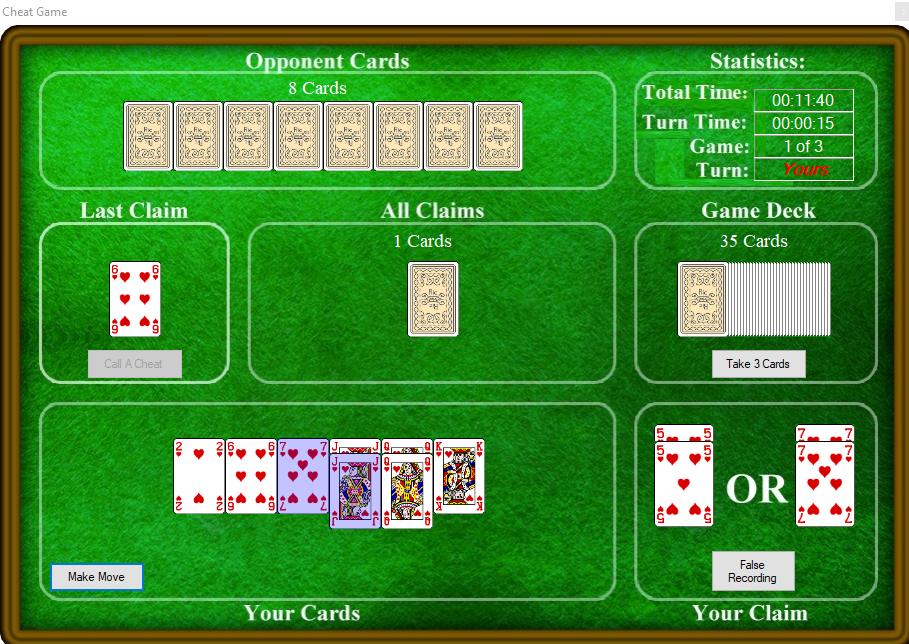
\includegraphics[width=4.5in]{Chapters/cheat_game_GUI}
	\caption{The graphical interfaced developed for the ``cheat game''.}
	\label{fig:cheatgamegui}
\end{figure}








%----------------------------------------------------------------------------------------
%	THESIS CONTENT - APPENDICES
%----------------------------------------------------------------------------------------

\appendix % Cue to tell LaTeX that the following "chapters" are Appendices

% Include the appendices of the thesis as separate files from the Appendices folder
% Uncomment the lines as you write the Appendices

% Appendix A

\chapter{Frequently Asked Questions} % Main appendix title

\label{AppendixA} % For referencing this appendix elsewhere, use \ref{AppendixA}

\section{How do I change the colors of links?}

The color of links can be changed to your liking using:

{\small\verb!\hypersetup{urlcolor=red}!}, or

{\small\verb!\hypersetup{citecolor=green}!}, or

{\small\verb!\hypersetup{allcolor=blue}!}.

\noindent If you want to completely hide the links, you can use:

{\small\verb!\hypersetup{allcolors=.}!}, or even better: 

{\small\verb!\hypersetup{hidelinks}!}.

\noindent If you want to have obvious links in the PDF but not the printed text, use:

{\small\verb!\hypersetup{colorlinks=false}!}.



%----------------------------------------------------------------------------------------
%	BIBLIOGRAPHY
%-----------------------------------------------------------------------
\printbibliography[heading=bibintoc]

%----------------------------------------------------------------------------------------

\end{document}  
